\documentclass[12pt]{report}
\usepackage[utf8]{inputenc}
\usepackage[russian]{babel}
%\usepackage[14pt]{extsizes}
\usepackage{listings}
\usepackage{graphicx}
\usepackage{amsmath,amsfonts,amssymb,amsthm,mathtools} 
\usepackage{pgfplots}
\usepackage{filecontents}
\usepackage{float}
\usepackage{comment}
\usepackage{indentfirst}
\usepackage{eucal}
\usepackage{enumitem}
%s\documentclass[openany]{book}
\frenchspacing

\usepackage{indentfirst} % Красная строка

\usetikzlibrary{datavisualization}
\usetikzlibrary{datavisualization.formats.functions}

\usepackage{amsmath}


% Для листинга кода:
% \lstset{ %
% 	language=c,                 % выбор языка для подсветки (здесь это С)
% 	basicstyle=\small\sffamily, % размер и начертание шрифта для подсветки кода
% 	numbers=left,               % где поставить нумерацию строк (слева\справа)
% 	numberstyle=\tiny,           % размер шрифта для номеров строк
% 	stepnumber=1,                   % размер шага между двумя номерами строк
% 	numbersep=5pt,                % как далеко отстоят номера строк от подсвечиваемого кода
% 	showspaces=false,            % показывать или нет пробелы специальными отступами
% 	showstringspaces=false,      % показывать или нет пробелы в строках
% 	showtabs=false,             % показывать или нет табуляцию в строках
% 	frame=single,              % рисовать рамку вокруг кода
% 	tabsize=2,                 % размер табуляции по умолчанию равен 2 пробелам
% 	captionpos=t,              % позиция заголовка вверху [t] или внизу [b] 
% 	breaklines=true,           % автоматически переносить строки (да\нет)
% 	breakatwhitespace=false, % переносить строки только если есть пробел
% 	escapeinside={\#*}{*)}   % если нужно добавить комментарии в коде
% }



\lstset{
    language=c,
    basicstyle= \footnotesize,
    breakatwhitespace=true,
    breaklines=true,
    inputencoding=utf8,
    numbers=left,
    numberstyle=\footnotesize,
    showspaces=false,
    showstringspaces=false,
    showtabs=false,
    stepnumber=1,
    tabsize=4,
    frame=single,
    escapebegin=\begin{russian}\commentfont,
    escapeend=\end{russian},
    literate={Ö}{{\"O}}1
    {Ä}{{\"A}}1
    {Ü}{{\"U}}1
    {ß}{{\ss}}1
    {ü}{{\"u}}1
    {ä}{{\"a}}1
    {ö}{{\"o}}1
    {~}{{\textasciitilde}}1
    {а}{{\selectfont\char224}}1
    {б}{{\selectfont\char225}}1
    {в}{{\selectfont\char226}}1
    {г}{{\selectfont\char227}}1
    {д}{{\selectfont\char228}}1
    {е}{{\selectfont\char229}}1
    {ё}{{\"e}}1
    {ж}{{\selectfont\char230}}1
    {з}{{\selectfont\char231}}1
    {и}{{\selectfont\char232}}1
    {й}{{\selectfont\char233}}1
    {к}{{\selectfont\char234}}1
    {л}{{\selectfont\char235}}1
    {м}{{\selectfont\char236}}1
    {н}{{\selectfont\char237}}1
    {о}{{\selectfont\char238}}1
    {п}{{\selectfont\char239}}1
    {р}{{\selectfont\char240}}1
    {с}{{\selectfont\char241}}1
    {т}{{\selectfont\char242}}1
    {у}{{\selectfont\char243}}1
    {ф}{{\selectfont\char244}}1
    {х}{{\selectfont\char245}}1
    {ц}{{\selectfont\char246}}1
    {ч}{{\selectfont\char247}}1
    {ш}{{\selectfont\char248}}1
    {щ}{{\selectfont\char249}}1
    {ъ}{{\selectfont\char250}}1
    {ы}{{\selectfont\char251}}1
    {ь}{{\selectfont\char252}}1
    {э}{{\selectfont\char253}}1
    {ю}{{\selectfont\char254}}1
    {я}{{\selectfont\char255}}1
    {А}{{\selectfont\char192}}1
    {Б}{{\selectfont\char193}}1
    {В}{{\selectfont\char194}}1
    {Г}{{\selectfont\char195}}1
    {Д}{{\selectfont\char196}}1
    {Е}{{\selectfont\char197}}1
    {Ё}{{\"E}}1
    {Ж}{{\selectfont\char198}}1
    {З}{{\selectfont\char199}}1
    {И}{{\selectfont\char200}}1
    {Й}{{\selectfont\char201}}1
    {К}{{\selectfont\char202}}1
    {Л}{{\selectfont\char203}}1
    {М}{{\selectfont\char204}}1
    {Н}{{\selectfont\char205}}1
    {О}{{\selectfont\char206}}1
    {П}{{\selectfont\char207}}1
    {Р}{{\selectfont\char208}}1
    {С}{{\selectfont\char209}}1
    {Т}{{\selectfont\char210}}1
    {У}{{\selectfont\char211}}1
    {Ф}{{\selectfont\char212}}1
    {Х}{{\selectfont\char213}}1
    {Ц}{{\selectfont\char214}}1
    {Ч}{{\selectfont\char215}}1
    {Ш}{{\selectfont\char216}}1
    {Щ}{{\selectfont\char217}}1
    {Ъ}{{\selectfont\char218}}1
    {Ы}{{\selectfont\char219}}1
    {Ь}{{\selectfont\char220}}1
    {Э}{{\selectfont\char221}}1
    {Ю}{{\selectfont\char222}}1
    {Я}{{\selectfont\char223}}1
    {і}{{\selectfont\char105}}1
    {ї}{{\selectfont\char168}}1
    {є}{{\selectfont\char185}}1
    {ґ}{{\selectfont\char160}}1
    {І}{{\selectfont\char73}}1
    {Ї}{{\selectfont\char136}}1
    {Є}{{\selectfont\char153}}1
    {Ґ}{{\selectfont\char128}}1
}


\usepackage[left=2cm,right=2cm, top=2cm,bottom=2cm,bindingoffset=0cm]{geometry}
% Для измененных титулов глав:
\usepackage{titlesec, blindtext, color} % подключаем нужные пакеты
\definecolor{gray75}{gray}{0.75} % определяем цвет
\newcommand{\hsp}{\hspace{20pt}} % длина линии в 20pt
% titleformat определяет стиль
\titleformat{\chapter}[hang]{\Huge\bfseries}{\thechapter\hsp\textcolor{gray75}{|}\hsp}{0pt}{\Huge\bfseries}


% plot
\usepackage{pgfplots}
\usepackage{filecontents}
\usetikzlibrary{datavisualization}
\usetikzlibrary{datavisualization.formats.functions}

\begin{document}
	%\def\chaptername{} % убирает "Глава"
	\thispagestyle{empty}
	\begin{titlepage}
		\noindent \begin{minipage}{0.15\textwidth}
			
\includegraphics[width=\linewidth]{img/b_logo}
		\end{minipage}
		\noindent\begin{minipage}{0.9\textwidth}\centering
			\textbf{Министерство науки и высшего образования Российской Федерации}\\
			\textbf{Федеральное государственное бюджетное образовательное учреждение высшего образования}\\
			\textbf{~~~«Московский государственный технический университет имени Н.Э.~Баумана}\\
			\textbf{(национальный исследовательский университет)»}\\
			\textbf{(МГТУ им. Н.Э.~Баумана)}
		\end{minipage}
		
		\noindent\rule{18cm}{3pt}
		\newline\newline
		\noindent ФАКУЛЬТЕТ $\underline{\text{«Информатика и системы управления»}}$ \newline\newline
		\noindent КАФЕДРА $\underline{\text{«Программное обеспечение ЭВМ и информационные технологии»}}$\newline\newline\newline\newline\newline
		
		\begin{center}
			\noindent\begin{minipage}{1.1\textwidth}\centering
				\Large\textbf{  Отчет по лабораторной работе №2}\newline
				\textbf{по дисциплине <<Математическая статистика>>}\newline\newline\newline\newline
			\end{minipage}
		\end{center}
		
		\noindent\textbf{Тема} $\underline{\text{Интервальные оценки~~~~~~}}$\newline\newline
		\noindent\textbf{Студент} $\underline{\text{Криков А.В.~~~~~~~~~~~~}}$\newline\newline
		\noindent\textbf{Группа} $\underline{\text{ИУ7-63Б~~~~~~~~~~~~~~~~~~~~~}}$\newline\newline
		\noindent\textbf{Оценка (баллы)} $\underline{\text{~~~~~~~~~~~~~~~~~~~}}$\newline\newline
		\noindent\textbf{Преподаватель} $\underline{\text{Власов П. А.}}$\newline\newline\newline
		
		\begin{center}
			\vfill
			Москва~---~\the\year
			~г.
		\end{center}
	\end{titlepage}

\chapter*{Задание}

\section*{Цель работы}
Построение доверительных интервалов для математического ожидания и дисперсии нормальной случайной величины.

\section*{Постановка задачи}

\begin{enumerate}
	\item Для выборки объема $n$ из нормальной генеральной совокупности $X$ реализовать в виде программы на ЭВМ
	\begin{enumerate}
		\item вычисление точечных оценок $\hat\mu(\vec X_n)$ и $S^2(\vec X_n)$ математического ожидания $MX$ и дисперсии $DX$ соответственно;
		\item вычисление нижней и верхней границ $\underline\mu(\vec X_n)$, $\overline\mu(\vec X_n)$ для $\gamma$-доверительного интервала для математического ожидания $MX$;
		\item вычисление нижней и верхней границ $\underline\sigma^2(\vec X_n)$, $\overline\sigma^2(\vec X_n)$ для $\gamma$-доверительного интервала для дисперсии $DX$;
	\end{enumerate}
	\item вычислить $\hat\mu$ и $S^2$ для выборки из индивидуального варианта;
	\item для заданного пользователем уровня доверия $\gamma$ и $N$ – объёма выборки из индивидуального варианта:
	\begin{enumerate}
		\item на координатной плоскости $Oyn$ построить прямую $y = \hat\mu(\vec{x_N})$, также графики функций $y = \hat\mu(\vec x_n)$, $y = \underline\mu(\vec x_n)$ и $y = \overline\mu(\vec x_n)$ как функций объема $n$ выборки, где $n$ изменяется от 1 до $N$;
		\item на другой координатной плоскости $Ozn$ построить прямую $z = S^2(\vec{x_N})$, также графики функций $z = S^2(\vec x_n)$, $z = \underline\sigma^2(\vec x_n)$ и $z = \overline\sigma^2(\vec x_n)$ как функций объема $n$ выборки, где $n$ изменяется от 1 до $N$.
	\end{enumerate}
\end{enumerate}

\chapter*{Теоретические сведения}

\section*{Определение $\gamma$-доверительного интервала для значения параметра распределения случайной величины}

Дана случайная величина $X$, закон распределения которой известен с точностью до неизвестного параметра $\theta$.

Интервальной оценкой с уровнем доверия $\gamma$ ($\gamma$-доверительной интервальной оценкой) параметра $\theta$ называют пару статистик $\underline{\theta}(\vec X), \overline{\theta}(\vec X)$ таких, что

\begin{equation*}
	P\{\underline{\theta}(\vec X)<\theta<\overline{\theta}(\vec X)\}=\gamma
\end{equation*}

Поскольку границы интервала являются случайными величинами, то для различных реализаций случайной выборки $\vec X$ статистики $\underline{\theta}(\vec X), \overline{\theta}(\vec X)$ могут принимать различные значения.

Доверительным интервалом с уровнем доверия $\gamma$ ($\gamma$-доверительным интервалом) называют интервал $(\underline{\theta}(\vec x), \overline{\theta}(\vec x))$, отвечающий выборочным значениям статистик $\underline{\theta}(\vec X), \overline{\theta}(\vec X)$.

\section*{Формулы для вычисления границ $\gamma$-доверительного \\ интервала для математического ожидания и дисперсии нормальной случайной величины}

Формулы для вычисления границ $\gamma$-доверительного интервала для математического ожидания:

\begin{equation}
\underline\mu(\vec X_n)=\overline X - \frac{S(\vec X)t^{St(n-1)}_{\frac{1+\gamma}{2}}}{\sqrt{n}}
\end{equation}

\begin{equation}
\overline\mu(\vec X_n)=\overline X + \frac{S(\vec X)t^{St(n-1)}_{\frac{1+\gamma}{2}}}{\sqrt{n}}
\end{equation}

$\overline X$ -- точечная оценка математического ожидания;

$S(\vec X) = \sqrtsign{S^2(\vec X)}$ -- квадратный корень из точечной оценки дисперсии;

$n$ -- объем выборки;

$\gamma$ -- уровень доверия;

$t^{St(n-1)}_{\alpha}$ -- квантиль уровня $\alpha$ распределения Стьюдента с $n - 1$ степенями свободы.
\newpage
Формулы для вычисления границ $\gamma$-доверительного интервала для дисперсии:

\begin{equation}
\underline\sigma(\vec X_n)= \frac{(n-1)S^2(\vec X)}{t^{\chi^2(n-1)}_{\frac{1+\gamma}{2}}}
\end{equation}

\begin{equation}
\overline\sigma(\vec X_n)= \frac{(n-1)S^2(\vec X)}{t^{\chi^2(n-1)}_{\frac{1-\gamma}{2}}}
\end{equation}

$S^2(\vec X)$ -- точечная оценка дисперсии;

$n$ -- объем выборки;

$\gamma$ -- уровень доверия;

$t^{\chi^2(n-1)}_{\alpha}$ -- квантиль уровня $\alpha$ распределения $\chi^2(n-1)$ с $n - 1$ степенями свободы.



\chapter*{Код программы}

\begin{lstlisting}[language=Matlab]
% Вариант 11

function lab()
	clc
	X =[
			-2.54,-0.79,-4.27,-3.09,-3.82,-0.61,...
			-0.64,-1.24,-1.73,-2.91,-1.48,-1.28,...
			-0.37,-1.88,-2.19,-1.61,-1.52,-3.17,...
			-1.36,-3.08,-3.11,-3.07,-1.57,-1.51,...
			-2.37,-0.58,-3.05,-2.93,-1.01,-1.40,...
			-2.06,-3.05,-1.84,-1.24,-1.89,-2.06,...
			-1.59,-2.83,-1.07,-2.96,-3.17,-3.08,...
			-0.49,-3.11,-3.14,-2.30,-3.99,-1.56,...
			-1.28,-3.46,-2.63,-0.82,-2.18,-0.89,...
			-3.08,-1.13,-1.62,-1.06,-2.98,-1.55,...
			-1.49,-1.65,-1.45,-2.29,-0.85,-1.44,...
			-2.87,-2.40,-2.13,-3.52,-1.42,-3.64,...
			-3.47,-2.05,-2.39,-2.07,-0.80,-1.52,...
			-3.92,-2.22,-0.78,-2.60,-1.78,-1.61,...
			-1.65,-2.06,-3.33,-3.41,-1.97,-1.74,...
			-2.04,0.01,-1.37,-3.15,-2.35,-3.66,...
			-1.79,-2.56,-1.87,-1.06,-0.64,-2.49,...
			-1.85,-1.40,-0.86,-0.17,-0.62,-2.85,...
			-2.12,-1.17,-2.48,-1.65,-3.74,-2.87,...
			-3.15,-1.89,-1.34,-4.33,-0.96,-1.79];

	% Уровень доверия
	gamma = 0.9;

	% Объем выборки 
	n = length(X);

	% Оценка мат. ожидания 
	mu = sum(X) / n;
	
	% Исправленная выборочная дисперсия
	S2 = sum((X - mu).^ 2) / (n - 1);

	% Нижняя граница доверительного интервала для мат. ожидания
	muLow = findMuLow(n, mu, S2, gamma);
	% Верхняя граница доверительного интервала для мат. ожидания
	muHigh = findMuHigh(n, mu, S2, gamma);

	% Нижняя граница доверительного интервала для дисперсии
	S2Low = findS2Low(n, S2, gamma);
	% Верхняя граница доверительного интервала для дисперсии
	S2High = findS2High(n, S2, gamma);

	% Вывод полученных ранее значений
	fprintf('mu = %.4f\n', mu);
	fprintf('S2 = %.4f\n', S2);
	fprintf('muLow = %.4f\n', muLow);
	fprintf('muHigh = %.4f\n', muHigh);
	fprintf('S2Low = %.4f\n', S2Low);
	fprintf('S2High = %.4f\n', S2High);
	
	% Создание массивов точечных оценок
	muArray = zeros(1, n);
	S2Array = zeros(1, n);
	% Создание массивов границ доверительных интервалов
	muLowArray = zeros(1, n);
	muHighArray = zeros(1, n);
	S2LowArray = zeros(1, n);
	S2HighArray = zeros(1, n);
	
	for i = 1 : n
		mu = sum(X(1:i)) / i;
		S2 = sum((X(1:i) - mu).^ 2) / (i - 1);

		muArray(i) = mu;
		S2Array(i) = S2;
		
		muLowArray(i) = findMuLow(i, mu, S2, gamma);
		muHighArray(i) = findMuHigh(i, mu, S2, gamma);        
		S2LowArray(i) = findS2Low(i, S2, gamma);        
		S2HighArray(i) = findS2High(i, S2, gamma);
	end
	
	% Построение графиков
	plot(1 : n, [(zeros(1, n) + mu)', muArray', muLowArray', muHighArray']);
	xlabel('n');
	ylabel('y');
	legend('$\hat \mu(\vec x_N)$', '$\hat \mu(\vec x_n)$', ...
		'$\underline{\mu}(\vec x_n)$', '$\overline{\mu}(\vec x_n)$', ...
		'Interpreter', 'latex', 'FontSize', 18);
	figure;
	plot(1 : n, [(zeros(1, n) + S2)', S2Array', S2LowArray', S2HighArray']);
	xlabel('n');
	ylabel('z');
	legend('$\hat S^2(\vec x_N)$', '$\hat S^2(\vec x_n)$', ...
		'$\underline{\sigma}^2(\vec x_n)$', '$\overline{\sigma}^2(\vec x_n)$', ...
		'Interpreter', 'latex', 'FontSize', 18);
end

% Функция поиска нижней границы доверительного интервала для матожидания
function muLow = findMuLow(n, mu, S2, gamma)
	muLow = mu - sqrt(S2) * tinv((1 + gamma) / 2, n - 1) / sqrt(n);
end

% Функция поиска верхней границы доверительного интервала для матожидания
function muHigh = findMuHigh(n, mu, S2, gamma)
	muHigh = mu + sqrt(S2) * tinv((1 + gamma) / 2, n - 1) / sqrt(n);
end

% Функция поиска нижней границы доверительного интервала для дисперсии
function S2Low = findS2Low(n, S2, gamma)
	S2Low = ((n - 1) * S2) / chi2inv((1 + gamma) / 2, n - 1);
end

% Функция поиска верхней границы доверительного интервала для дисперсии
function S2High = findS2High(n, S2, gamma)
	S2High = ((n - 1) * S2) / chi2inv((1 - gamma) / 2, n - 1);
end
\end{lstlisting}

\section*{Результаты расчётов}
\begin{equation*}
	\hat\mu(\vec x_n) = -2,0585\\
\end{equation*}

\begin{equation*}
	S^2(\vec x_n) = 0,9440\\
\end{equation*}

\begin{equation*}
	\underline\mu(\vec x_n) = -2,2055\\
\end{equation*}

\begin{equation*}
	\overline\mu(\vec x_n) = -1,9115\\
\end{equation*}

\begin{equation*}
	\underline{S^2}(\vec x_n) = 0,7723\\
\end{equation*}

\begin{equation*}
	\overline{S^2}(\vec x_n) = 1,1848\\
\end{equation*}

\begin{figure}[h]
	\centering
	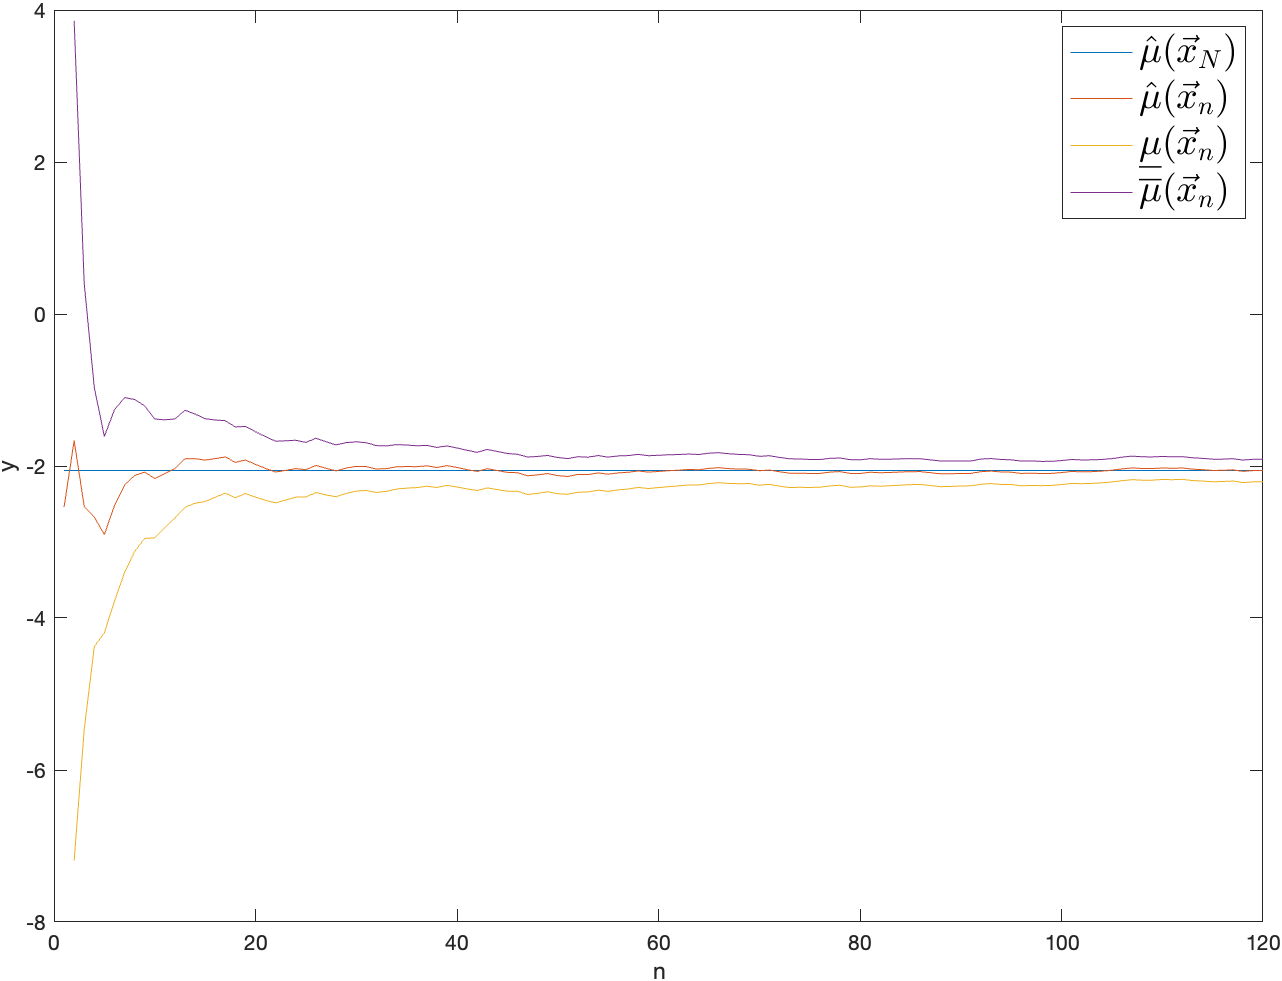
\includegraphics[scale=0.5]{img/1.png}
	\caption{Прямая $y(n) = \hat\mu(\vec x_N)$, а также графики функций $y(n) = \underline\mu(\vec x_n)$, $y(n) = \overline\mu(\vec x_n)$, $y(n) = \hat\mu(\vec x_n)$ как функций объема $n$ выборки, где $n$ изменяется от 1 до $N$}
	\label{fig:1}
\end{figure}

\begin{figure}[h]
	\centering
	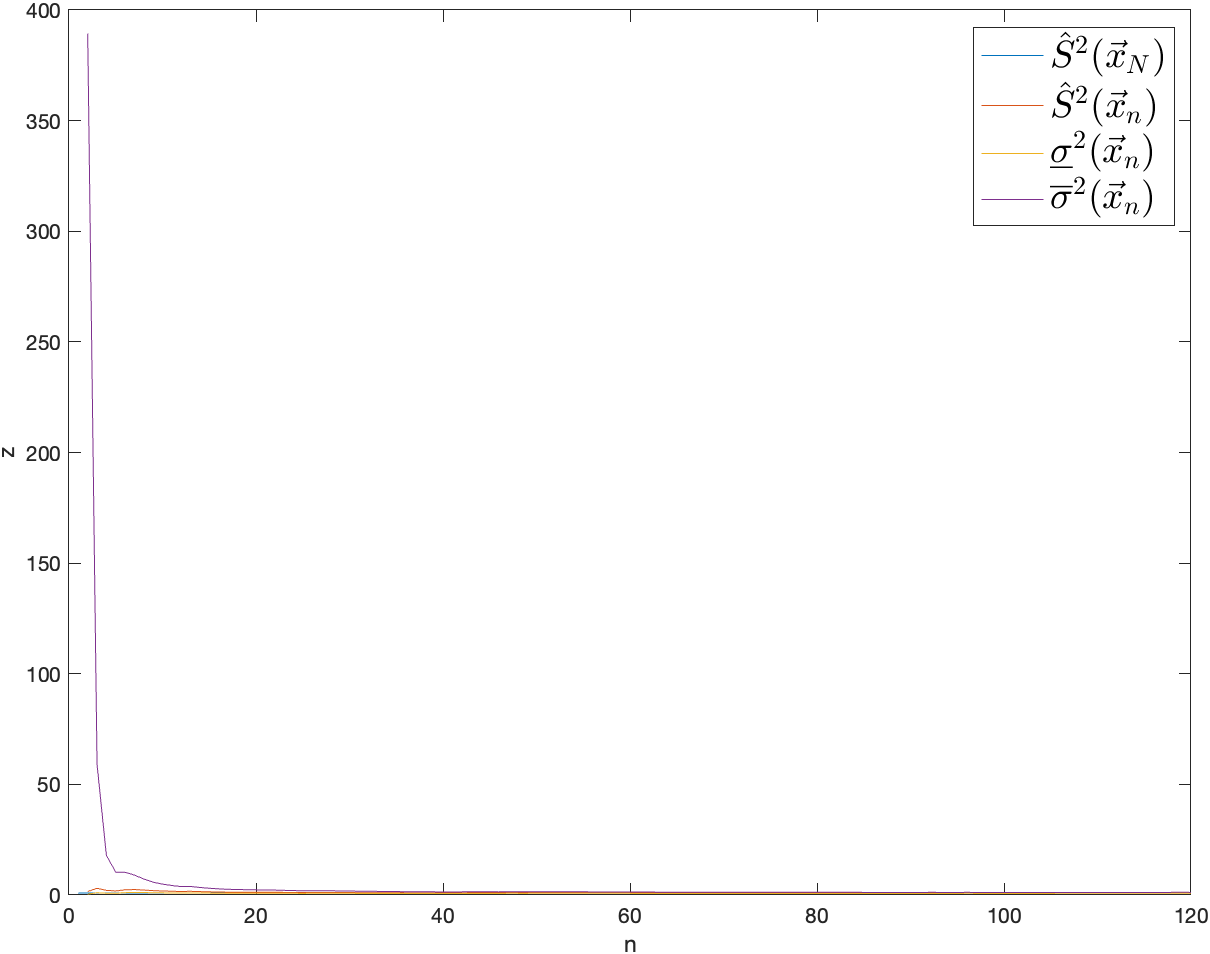
\includegraphics[scale=0.5]{img/2.png}
	\caption{Прямая $z(n) = \hat S^2(\vec x_N)$, а также графики функций $z(n) = \underline S^2(\vec x_n)$, $z(n) = \overline S^2(\vec x_n)$, $z(n) = \hat S^2(\vec x_n)$ как функций объема $n$ выборки, где $n$ изменяется от 1 до $N$}
	\label{fig:2}
\end{figure}

\begin{figure}[h]
	\centering
	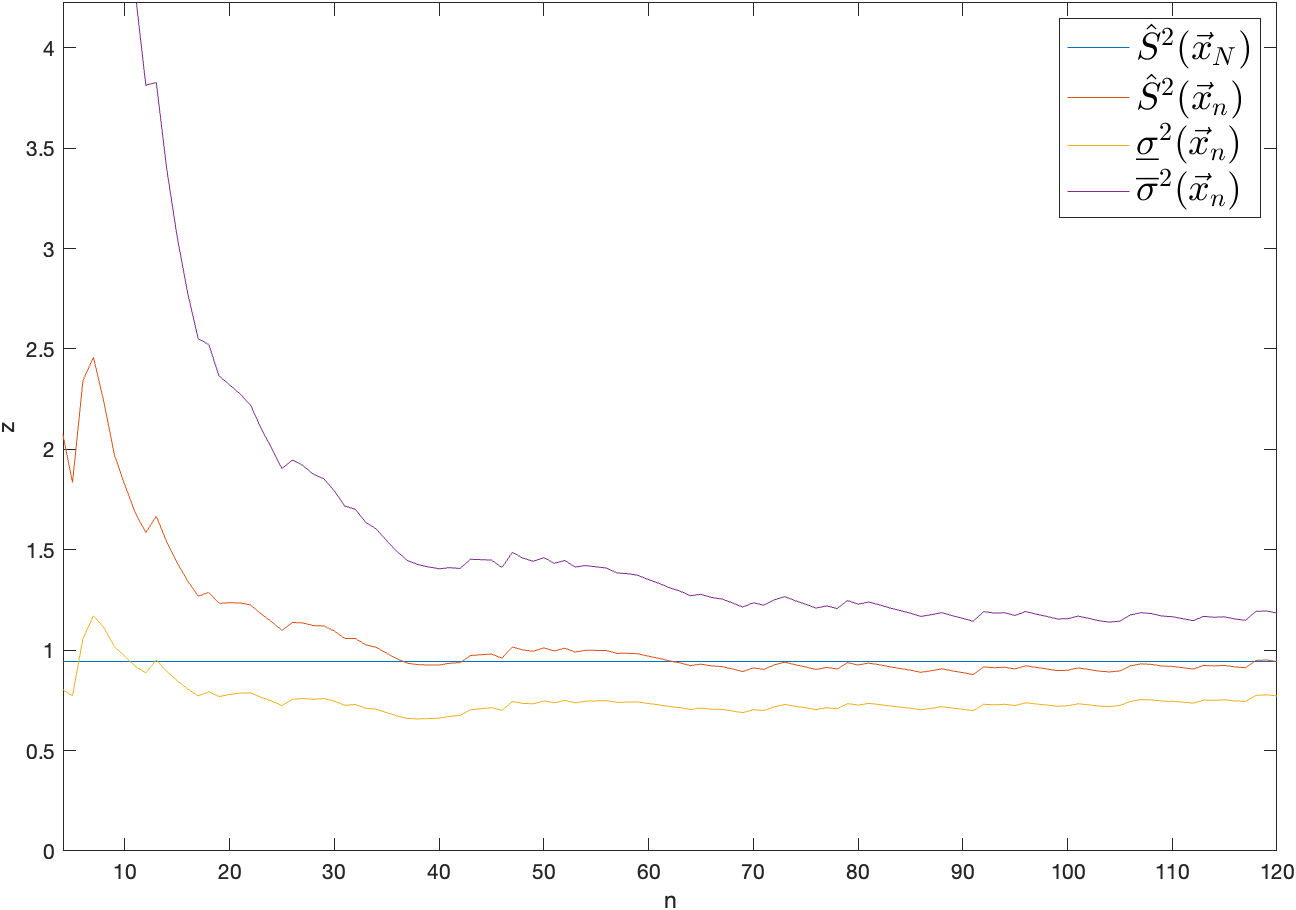
\includegraphics[scale=0.5]{img/3.png}
	\caption{Прямая $z(n) = \hat S^2(\vec x_N)$, а также графики функций $z(n) = \underline S^2(\vec x_n)$, $z(n) = \overline S^2(\vec x_n)$, $z(n) = \hat S^2(\vec x_n)$ как функций объема $n$ выборки, где $n$ изменяется от 1 до $N$ (приближенный)}
	\label{fig:3}
\end{figure}

\bibliographystyle{utf8gost705u}  % стилевой файл для оформления по ГОСТу
\bibliography{51-biblio}          % имя библиографической базы (bib-файла)
	
\end{document}